\tikzset{every picture/.style={line width=0.75pt}} %set default line width to 0.75pt        

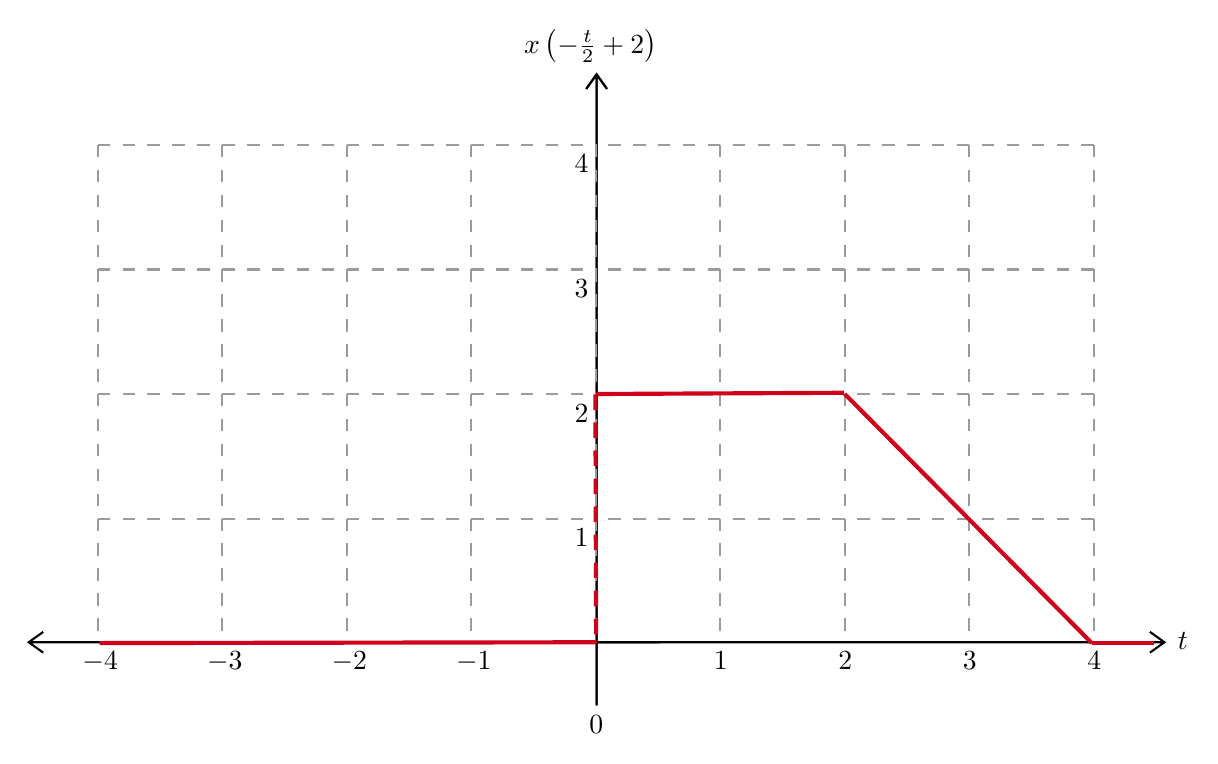
\begin{tikzpicture}[x=0.75pt,y=0.75pt,yscale=-1,xscale=1]
%uncomment if require: \path (0,423); %set diagram left start at 0, and has height of 423

%Shape: Axis 2D [id:dp7787745858917079] 
\draw  (314,335.6) -- (618,335.6)(344.4,62) -- (344.4,366) (611,330.6) -- (618,335.6) -- (611,340.6) (339.4,69) -- (344.4,62) -- (349.4,69)  ;
%Shape: Axis 2D [id:dp2833357045793793] 
\draw  (374.8,335.6) -- (70.8,335.6)(344.4,62) -- (344.4,366) (77.8,330.6) -- (70.8,335.6) -- (77.8,340.6) (349.4,69) -- (344.4,62) -- (339.4,69)  ;
%Shape: Grid [id:dp29542181740302487] 
\draw  [draw opacity=0][dash pattern={on 4.5pt off 4.5pt}] (104,96) -- (344.4,96) -- (344.4,334.7) -- (104,334.7) -- cycle ; \draw  [color={rgb, 255:red, 155; green, 155; blue, 155 }  ,draw opacity=1 ][dash pattern={on 4.5pt off 4.5pt}] (104,96) -- (104,334.7)(164,96) -- (164,334.7)(224,96) -- (224,334.7)(284,96) -- (284,334.7)(344,96) -- (344,334.7) ; \draw  [color={rgb, 255:red, 155; green, 155; blue, 155 }  ,draw opacity=1 ][dash pattern={on 4.5pt off 4.5pt}] (104,96) -- (344.4,96)(104,156) -- (344.4,156)(104,216) -- (344.4,216)(104,276) -- (344.4,276) ; \draw  [color={rgb, 255:red, 155; green, 155; blue, 155 }  ,draw opacity=1 ][dash pattern={on 4.5pt off 4.5pt}]  ;
%Shape: Grid [id:dp6629033718892944] 
\draw  [draw opacity=0][dash pattern={on 4.5pt off 4.5pt}] (584,96) -- (343.6,96) -- (343.6,334) -- (584,334) -- cycle ; \draw  [color={rgb, 255:red, 155; green, 155; blue, 155 }  ,draw opacity=1 ][dash pattern={on 4.5pt off 4.5pt}] (584,96) -- (584,334)(524,96) -- (524,334)(464,96) -- (464,334)(404,96) -- (404,334)(344,96) -- (344,334) ; \draw  [color={rgb, 255:red, 155; green, 155; blue, 155 }  ,draw opacity=1 ][dash pattern={on 4.5pt off 4.5pt}] (584,96) -- (343.6,96)(584,156) -- (343.6,156)(584,216) -- (343.6,216)(584,276) -- (343.6,276) ; \draw  [color={rgb, 255:red, 155; green, 155; blue, 155 }  ,draw opacity=1 ][dash pattern={on 4.5pt off 4.5pt}]  ;
%Straight Lines [id:da7162297428339012] 
\draw [color={rgb, 255:red, 208; green, 2; blue, 27 }  ,draw opacity=1 ][line width=1.5]    (105,336) -- (344.4,335.6) ;
%Straight Lines [id:da6489949529763962] 
\draw [color={rgb, 255:red, 208; green, 2; blue, 27 }  ,draw opacity=1 ][line width=1.5]    (583,336) -- (464,216) ;
%Straight Lines [id:da23798784359213232] 
\draw [color={rgb, 255:red, 208; green, 2; blue, 27 }  ,draw opacity=1 ][line width=1.5]    (344,216) -- (463.6,215.4) ;
%Straight Lines [id:da3244245846200695] 
\draw [color={rgb, 255:red, 208; green, 2; blue, 27 }  ,draw opacity=1 ][line width=1.5]    (583,336) -- (613,336) ;
%Straight Lines [id:da5286072330399609] 
\draw [color={rgb, 255:red, 208; green, 2; blue, 27 }  ,draw opacity=1 ][line width=1.5]  [dash pattern={on 5.63pt off 4.5pt}]  (343.82,216.2) -- (344.18,335.8) ;

% Text Node
\draw (344.23,369.4) node [anchor=north] [inner sep=0.75pt]    {$0$};
% Text Node
\draw (404.23,338.4) node [anchor=north] [inner sep=0.75pt]    {$1$};
% Text Node
\draw (464.23,338.4) node [anchor=north] [inner sep=0.75pt]    {$2$};
% Text Node
\draw (524.23,338.4) node [anchor=north] [inner sep=0.75pt]    {$3$};
% Text Node
\draw (584.23,338.4) node [anchor=north] [inner sep=0.75pt]    {$4$};
% Text Node
\draw (105.23,338.4) node [anchor=north] [inner sep=0.75pt]    {$-4$};
% Text Node
\draw (165.23,338.4) node [anchor=north] [inner sep=0.75pt]    {$-3$};
% Text Node
\draw (225.23,338.4) node [anchor=north] [inner sep=0.75pt]    {$-2$};
% Text Node
\draw (285.23,338.4) node [anchor=north] [inner sep=0.75pt]    {$-1$};
% Text Node
\draw (342,279.4) node [anchor=north east] [inner sep=0.75pt]    {$1$};
% Text Node
\draw (342,219.4) node [anchor=north east] [inner sep=0.75pt]    {$2$};
% Text Node
\draw (342,159.4) node [anchor=north east] [inner sep=0.75pt]    {$3$};
% Text Node
\draw (342,99.4) node [anchor=north east] [inner sep=0.75pt]    {$4$};
% Text Node
\draw (308,58) node [anchor=south west] [inner sep=0.75pt]    {$x\left( -\frac{t}{2} +2\right)$};
% Text Node
\draw (623,329.4) node [anchor=north west][inner sep=0.75pt]    {$t$};


\end{tikzpicture}
